\subsection{Cargueiros comerciais}

A espaçonave SpaceX Dragon desempenha um papel crucial no transporte de cargas essenciais e na devolução de experimentos científicos da Estação Espacial Internacional (ISS) para a Terra. Em sua mais recente missão, a Dragon retornou com sucesso, trazendo resultados de pesquisas críticas conduzidas em ambiente de microgravidade. Este retorno marca mais um marco na parceria entre a NASA e a SpaceX para a condução de missões científicas e logísticas em órbita terrestre \citep{nasaDragonReturn}.

A capacidade única da Dragon de retornar cargas à Terra a torna indispensável para a realização de estudos científicos avançados. Durante algumas missões, ela trouxe uma carga significativa de experimentos e dados científicos, incluindo pesquisas em biologia, como explicado por \citep{bell2018}, ciência dos materiais conforme o estudo realizado por \citep{chamberlain2021} e fisiologia humana, como escrito por \citep{wang2018}. Esses resultados são essenciais para avançar na compreensão dos desafios de missões espaciais de longa duração, como aquelas planejadas para a Lua e Marte \citep{nasaDragonReturn}.

Além do transporte de cargas científicas, a Dragon demonstrou avanços em tecnologias de reentrada e aterrissagem seguras e de forma que possam reutilizar o mesmo equipamento para missões futuras, como descrito por \citep{nasaFalcon9Dragon}. Após se desacoplar da ISS, como escrito por \citep{nasaspaceflightDroneShip}, a espaçonave reentrou na atmosfera terrestre e pousou em uma plataforma drone retangular no Oceano Pacífico. A comprovada confiabilidade e a capacidade de operar de forma consistente do sistema Dragon consolidam sua posição como um veículo indispensável para transporte e pesquisa científica na ISS \citep{nasaDragonReturn}.

\subsection{Autonomia no docking da espaçonave Dragon}

A espaçonave Dragon da SpaceX utiliza tecnologias avançadas, como explicado por \citep{nasaspaceflightDragonISS}, de LIDAR e GPS para realizar manobras autônomas até a Estação Espacial Internacional (ISS). O LIDAR fornece medições tridimensionais precisas da distância e orientação em relação à ISS, permitindo que a Dragon ajuste continuamente sua posição durante as fases críticas de aproximação. Simultaneamente, o sistema GPS integrado oferece dados de localização em tempo real, garantindo alinhamento com a trajetória orbital da estação.

Essas tecnologias trabalham em conjunto para permitir que a Dragon alcance o ponto de captura designado com mínima intervenção humana. Uma vez em posição, o braço robótico Canadarm2, operado pelos astronautas a bordo da ISS, é utilizado para capturar e conectar a Dragon ao porto de acoplamento. Ainda que tenha supervisão humana, esse processo garante segurança e eficiência nas operações orbitais, reduzindo erros e prejuízos a operação.

\begin{figure}[H]
    \centering
    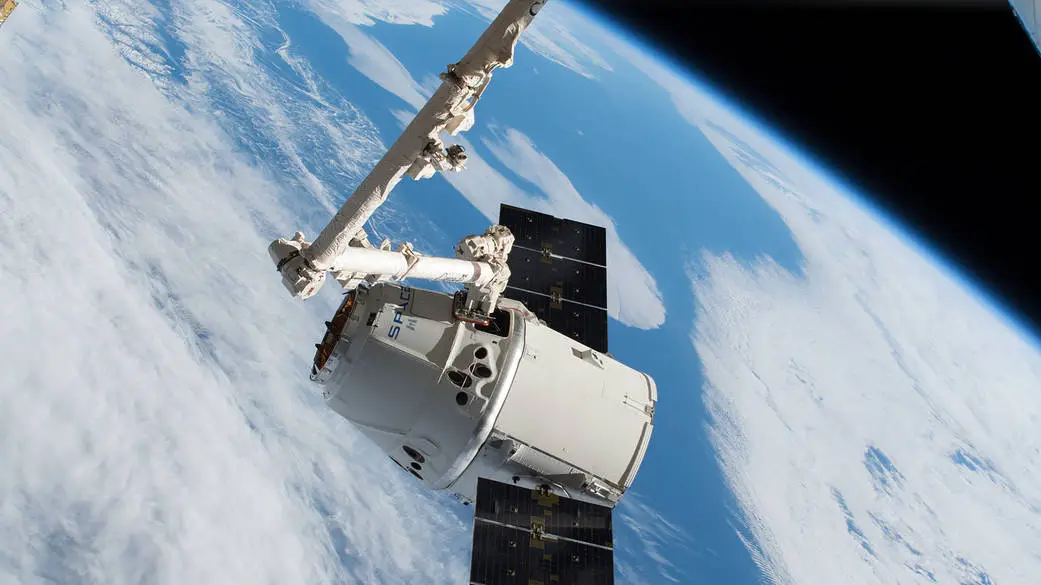
\includegraphics[width=0.75\linewidth]{Imagens/SpaceX Dragon Canadarm2 foto 1.png}
    \caption{Espaçonave Dragon da SpaceX sendo capturada pelo Canadarm2. Fonte: Nasa (\url{https://www.nasa.gov/image-article/spacex-dragon-captured-with-canadarm2}).}
    \label{fig:DragonCadanarm2Foto}
\end{figure}


